%%%%%%%%%%%%%%%%%%%%%%%%%%%%%%%%%%%%%%%%%%%%%%%%%%%%%%%%%%%%%%%%%%%%%%%%%%%%%%
%% Lecture 2: Visualization and Matplotlib.
%% Compile with: latexmk -pdf lecture02
%% Handout (overlays collapsed, solutions shown): latexmk -pdf lecture02-handout
%% Speaker notes: add the notes option to \usepackage below.
%%
%% Data and figures: ../codes/l02_figures.py (run with uv run codes/l02_figures.py).
%% Based on the 2025 slides of Stevan Rudinac and on Lecture 3 of Andreas
%% Mueller's Applied Machine Learning course (Columbia University, 2017).
%%%%%%%%%%%%%%%%%%%%%%%%%%%%%%%%%%%%%%%%%%%%%%%%%%%%%%%%%%%%%%%%%%%%%%%%%%%%%%

% lecture02-handout.tex defines \sibhandout before reading this file.
\ifdefined\sibhandout
  \documentclass[handout,aspectratio=169,t,9pt]{beamer}
  \usepackage[macros,solutions]{siblecture2026}
\else
  \documentclass[aspectratio=169,t,9pt]{beamer}
  \usepackage[macros]{siblecture2026}
\fi

% Everything specific to this course goes here.
\graphicspath{{figures/}{../images/}}
\usepackage{booktabs}
\usepackage{listings}
\lstset{language=Python,
        basicstyle=\ttfamily\footnotesize,
        keywordstyle=\color{sibTwo}\bfseries,
        stringstyle=\color{sibOne},
        commentstyle=\color{uvaDarkGrey},
        backgroundcolor=\color{uvaGrey},
        columns=fullflexible,keepspaces=true,showstringspaces=false,
        frame=none,xleftmargin=4pt,xrightmargin=4pt,
        aboveskip=4pt,belowskip=4pt}

%%%%%%%%%%%%%%%%%%%%%%%%%%%%%%%%%%%%%%%%%%%%%%%%%%%%%%%%%%%%%%%%%%%%%%%%%%%%%%

\course{Machine Learning with Python}
\coursesubtitle{Minor Amsterdam Data Science and Artificial Intelligence}
\term{Fall 2026}

\lectureno{2}
\title{Visualization and Matplotlib}
\subtitle{Look at your data before you model it}
\author{\c{S}. \.{I}lker Birbil}
\institute{University of Amsterdam}
\date{October 27, 2026}
\contact{s.i.birbil@uva.nl}

% ============================================================
\begin{document}
% ============================================================

\sibtitleframe

\sibtocframe[Lecture overview]

\begin{frame}{What you should be able to do afterwards}
  \begin{objectives}
    \item Explain why we plot the data before we model it.
    \item Recognize common data problems in a plot.
    \item Choose a chart and a colormap that fit the question.
    \item Read and write basic \texttt{matplotlib} code.
  \end{objectives}

  \vfill
  \begin{recap}
    Machine learning learns a rule from examples and is judged on new data.
    The workflow starts with the goal and with \emph{exploring the data}.
  \end{recap}
\end{frame}

% ==================================================================
\section{Why Visualize?}
% ==================================================================

\begin{frame}{Two reasons to make a plot}
  \vspace{0.3cm}
  \begin{columns}[T,onlytextwidth]
    \begin{column}{0.48\textwidth}
      \begin{sibbox}{Explore}
        For yourself: find patterns, errors and surprises.
      \end{sibbox}
    \end{column}
    \begin{column}{0.48\textwidth}
      \begin{sibbox}{Communicate}
        For others: show a finding clearly and honestly.
      \end{sibbox}
    \end{column}
  \end{columns}

  \vfill
  \begin{takeaway}
    In machine learning, exploring comes first: plots tell you which
    problems to fix and which models to try.
  \end{takeaway}

  \note{M\"{u}ller (2017) stresses exploration over presentation in this
    course.  Always ask what the point of a plot is, and whether the chart
    type serves that point.}
\end{frame}

\begin{frame}{Anscombe's quartet}
  \centering
  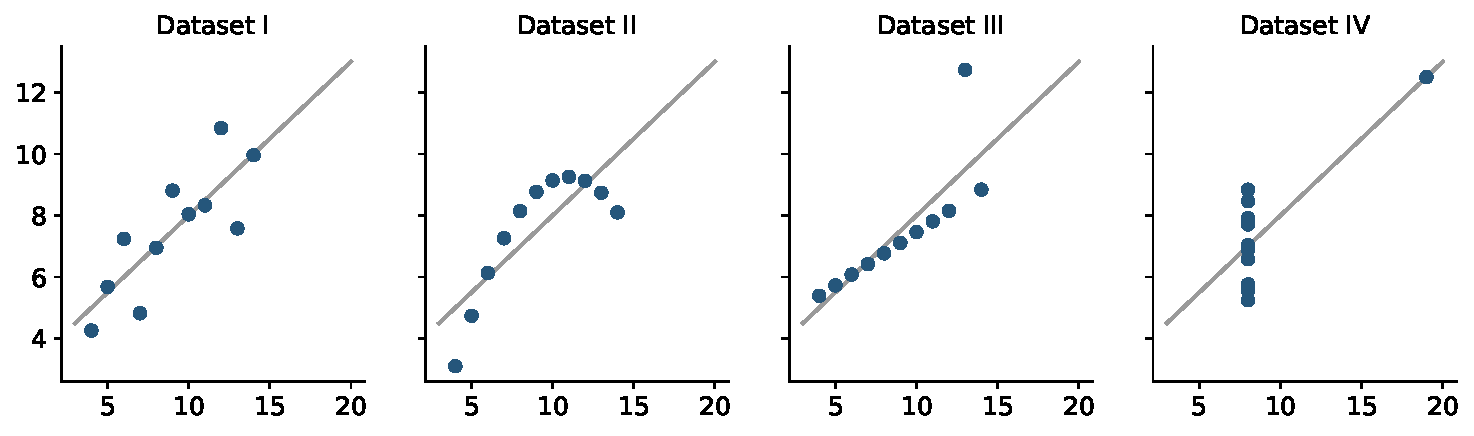
\includegraphics[width=0.94\textwidth]{l02_anscombe.pdf}

  \vspace{0.3cm}
  \raggedright
  All four datasets have the \highlight{same} means, variances,
  correlation ($0.82$) and regression line ($y = 3 + 0.5x$).

  \vfill
  \begin{keypoint}{Lesson}
    Summary statistics can hide the shape of the data.  Always plot it
    (Anscombe, 1973).
  \end{keypoint}

  \note{I: a linear relation with noise.  II: a curve.  III: a perfect line
    with one outlier.  IV: no relation at all, except one extreme point.
    A model fitted to the summary numbers alone treats them all the same.}
\end{frame}

% ==================================================================
\section{What a Plot Reveals}
% ==================================================================

\begin{frame}{Correlation is not causation}
  \begin{columns}[T,onlytextwidth]
    \begin{column}{0.58\textwidth}
      \centering
      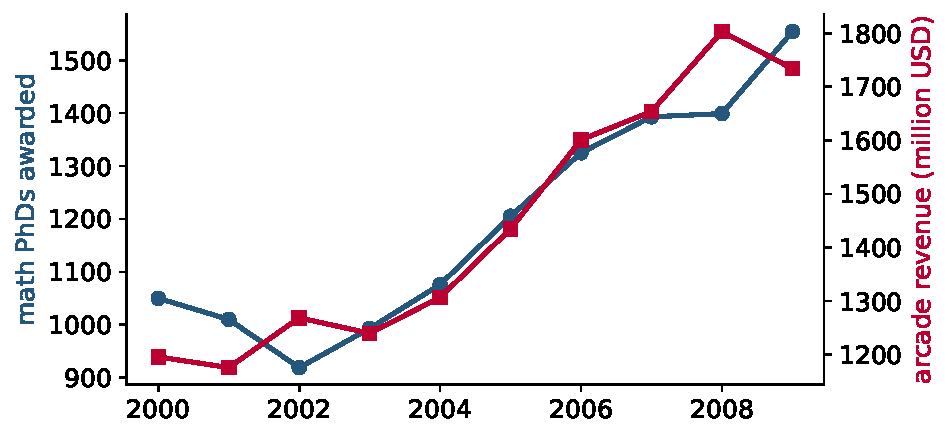
\includegraphics[width=\linewidth]{l02_spurious.pdf}
    \end{column}
    \begin{column}{0.38\textwidth}
      \vspace{0.3cm}
      \begin{itemize}
        \item Correlation: $0.94$
        \item Does arcade revenue produce mathematicians?
        \item Both simply grow over time.
      \end{itemize}
    \end{column}
  \end{columns}

  \vfill
  \muted{Data as used in M\"{u}ller (2017), after Vigen's \emph{Spurious
  Correlations}.}

  \note{Two series that both trend upward are always correlated.  A model
    may happily use such a feature; it will break as soon as the trends
    diverge.  The twin y-axes also make the match look closer than it is;
    we return to this in the second session.}
\end{frame}

\begin{frame}{Wrong data type}
  \centering
  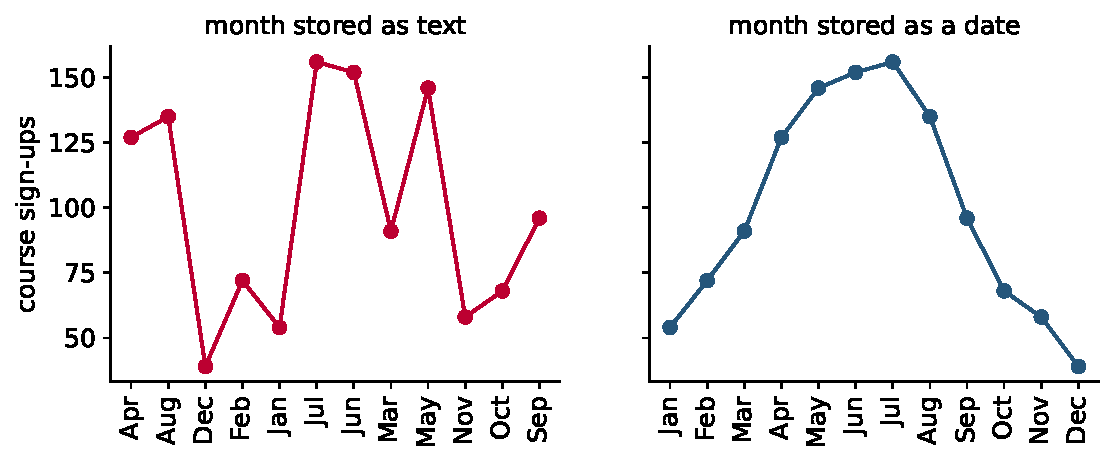
\includegraphics[height=3.5cm]{l02_datatype.pdf}

  \vspace{0.3cm}
  \raggedright
  Text is sorted alphabetically: Apr, Aug, Dec, \dots

  \vfill
  \begin{keypoint}{Check}
    Is every column stored as what it is: a number, a date, a category?
  \end{keypoint}

  \note{Synthetic illustration.  The same happens with numbers stored as
    text, for instance grades exported with a decimal comma: they cannot
    be averaged or plotted on a numeric axis.}
\end{frame}

\begin{frame}{Definition mismatch}
  \centering
  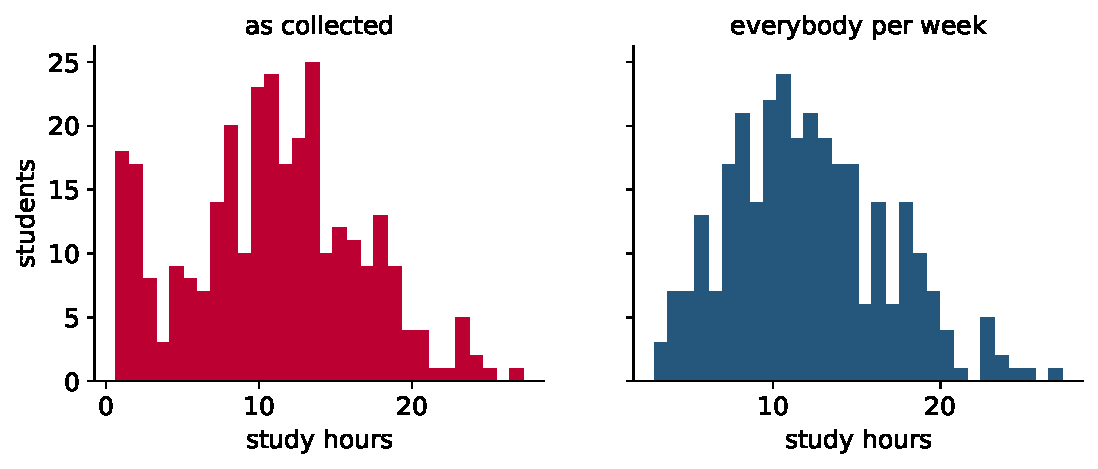
\includegraphics[height=3.5cm]{l02_definition.pdf}

  \vspace{0.3cm}
  \raggedright
  Some respondents reported study hours \highlight{per day}, others
  \highlight{per week}.

  \vfill
  \begin{keypoint}{Check}
    Does every value mean the same thing?  Two peaks often mean two
    definitions.
  \end{keypoint}

  \note{Synthetic illustration from the course survey.  Similar mismatches:
    prices with and without VAT, amounts in euros and in thousands of
    euros, ``income'' per month and per year.}
\end{frame}

\begin{frame}{Suspiciously round numbers}
  \begin{columns}[T,onlytextwidth]
    \begin{column}{0.56\textwidth}
      \centering
      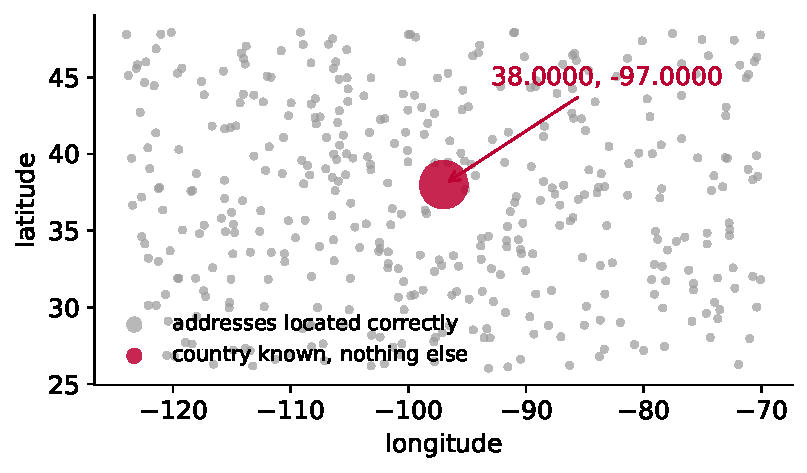
\includegraphics[width=\linewidth]{l02_kansas.pdf}
    \end{column}
    \begin{column}{0.40\textwidth}
      \begin{itemize}
        \item A database maps internet addresses to places.
        \item Country known, nothing else?  Use the default
              \highlight{38.0000, $-$97.0000}.
        \item That point is a farm in Kansas: more than 600 million
              addresses ended up there (Hill, 2016).
      \end{itemize}
    \end{column}
  \end{columns}

  \vfill
  \begin{keypoint}{Check}
    A pile-up at one round value is often a default, not a measurement.
  \end{keypoint}

  \note{The plot is a synthetic illustration; the case is real.  The
    residents were visited repeatedly by police and by people who believed
    their stolen devices or online fraudsters were there.  The company later
    moved the default point.  The same pattern appears as birthdays on
    January 1, ages of 99, or incomes of exactly 0.}
\end{frame}

% ==================================================================
\section{Principles of Good Plots}
% ==================================================================

\begin{frame}{Show the data}
  \vspace{0.3cm}
  \begin{columns}[T,onlytextwidth]
    \begin{column}{0.48\textwidth}
      \begin{sibbox}{Above all else, show the data}
        The data should stand out, not the decoration.
      \end{sibbox}
    \end{column}
    \begin{column}{0.48\textwidth}
      \begin{sibbox}{Maximize the data-ink ratio}
        Remove ink that does not depend on the data: 3D effects,
        heavy grids, shadows.
      \end{sibbox}
    \end{column}
  \end{columns}

  \vfill
  \muted{Both principles: Tufte (1983).}

  \note{Data ink is the ink that would change if the data changed.  Ask of
    every element of a plot: does it carry information?}
\end{frame}

\begin{frame}{Which bar is the largest?}
  \centering
  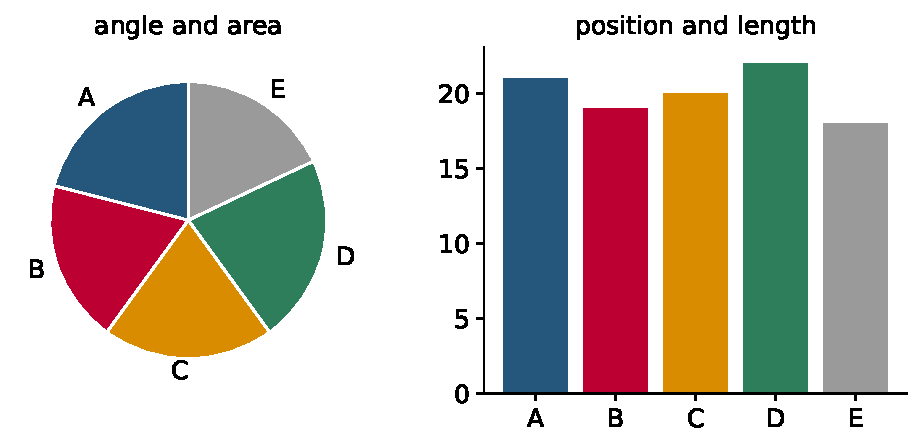
\includegraphics[height=3.8cm]{l02_channels.pdf}

  \vfill
  \begin{keypoint}{Visual channels, from most to least accurate}
    position $>$ length $>$ angle $>$ area $>$ color
    \hfill \muted{(after Cleveland and McGill, 1984)}
  \end{keypoint}

  \note{Ask the room which slice is largest before showing the bars.  The
    values are 21, 19, 20, 22 and 18: hard to rank in the pie, easy in the
    bars.  Hue is the weakest channel for quantities; use it for
    categories.}
\end{frame}

\begin{frame}{Three kinds of colormaps}
  \centering
  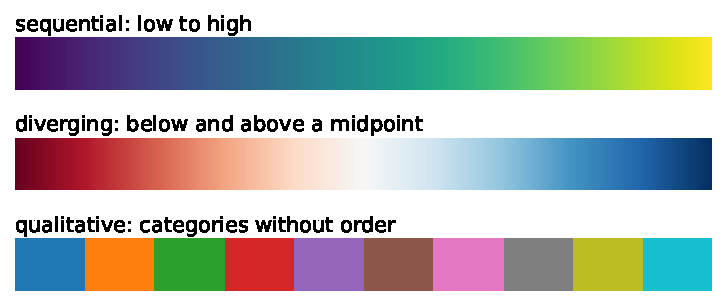
\includegraphics[width=0.7\textwidth]{l02_cmap_types.pdf}

  \vfill
  \raggedright
  \begin{itemize}
    \item \textbf{Sequential:} amounts, e.g., population density
    \item \textbf{Diverging:} deviations from a midpoint, e.g., profit and
          loss, correlations
    \item \textbf{Qualitative:} groups, e.g., study programs
  \end{itemize}
\end{frame}

\begin{frame}{Avoid the rainbow}
  \centering
  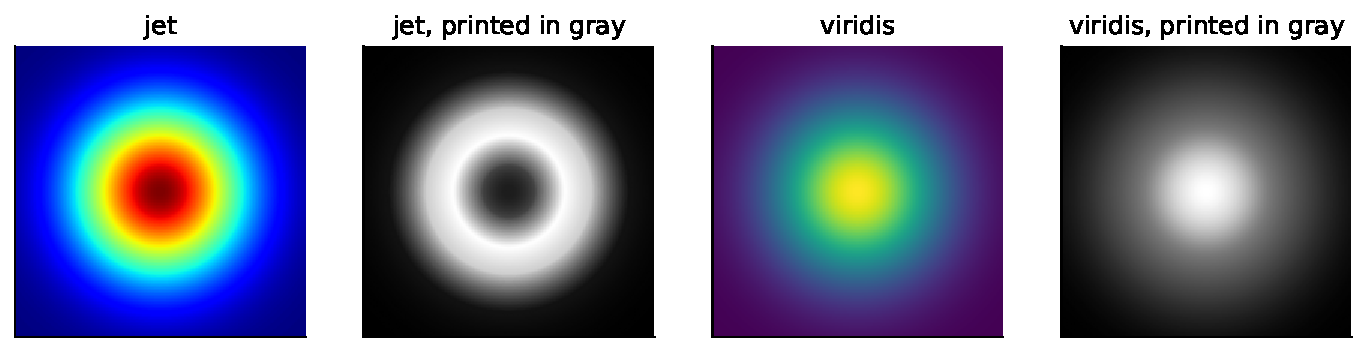
\includegraphics[width=\textwidth]{l02_colormaps.pdf}

  \vspace{0.3cm}
  \raggedright
  The same smooth data.  \texttt{jet} invents rings and loses its order in
  gray; \texttt{viridis} does neither.

  \vfill
  \muted{Borland and Taylor (2007); Smith and van der Walt (2015).}

  \note{Rainbow colormaps have sharp perceptual edges, so we see boundaries
    that are not in the data, and their brightness is not monotone, so a
    gray printout does not go from dark to light.  Viridis is the default
    in matplotlib since version 2.0.}
\end{frame}

\begin{frame}{Check your understanding}
  \begin{exercise}[which chart?]
    Pick a line plot, a scatter plot, a histogram or a bar chart.
    \begin{enumerate}[label=(\alph*),itemsep=2pt,topsep=3pt]
      \item How did weekly study hours change during the course?
      \item Do students who sleep more get higher grades?
      \item Which program has the highest average grade?
      \item How are the ages of the students distributed?
    \end{enumerate}
  \end{exercise}

  \begin{solution}
    (a) Line plot: a trend over time.
    (b) Scatter plot: the relation between two numbers.
    (c) Bar chart: one number per group.
    (d) Histogram: the distribution of one number.
  \end{solution}

  \note{One minute, then ask for answers.}
\end{frame}

% ==================================================================
\section{Plotting in Python}
% ==================================================================

\begin{frame}{The first session in one slide}
  \vspace{0.3cm}
  \begin{recap}[Where we are]
    \begin{itemize}
      \item Always plot the data: statistics can hide its shape.
      \item Plots reveal wrong types, mixed definitions and defaults.
      \item Use position and length; avoid rainbow colormaps.
    \end{itemize}
  \end{recap}

  \vspace{0.6cm}
  Now: \highlight{how to make these plots in Python}.
\end{frame}

\begin{frame}{Plotting libraries in Python}
  \vspace{0.3cm}
  \begin{tabular}{@{}ll@{}}
    \toprule
    \texttt{matplotlib} & the foundation; full control (Hunter, 2007) \\
    \texttt{pandas}     & quick plots of a table: \texttt{df.plot()} \\
    \texttt{seaborn}    & statistical plots in one line (Waskom, 2021) \\
    \texttt{plotly}, \texttt{bokeh} & interactive plots in the browser \\
    \bottomrule
  \end{tabular}

  \vfill
  \begin{takeaway}
    Learn \texttt{matplotlib} first: the others build on it or copy its
    ideas.
  \end{takeaway}

  \note{The laptop labs also use seaborn and bokeh.  In Jupyter, plots
    appear below the cell automatically.}
\end{frame}

\begin{frame}[fragile]{The course data: a student survey}
  \begin{lstlisting}
import pandas as pd
import matplotlib.pyplot as plt

df = pd.read_csv("student_survey.csv")
df.head()
  \end{lstlisting}

  \vspace{0.2cm}
  \begin{tabular}{@{}ll@{}}
    \toprule
    \texttt{program}            & Economics, Business, \dots \\
    \texttt{study\_hours}       & hours per week \\
    \texttt{social\_media\_hours} & hours per day \\
    \texttt{sleep\_hours}       & hours per night \\
    \texttt{grade}              & 1--10 \\
    \bottomrule
  \end{tabular}

  \vfill
  \muted{300 synthetic students; the file is in \texttt{codes/data/}.}

  \note{The survey also has age, satisfaction (1--5) and passed (grade at
    least 5.5).  The data are generated by the course script, so every
    figure in this lecture can be reproduced.}
\end{frame}

\begin{frame}[fragile]{Figures and axes}
  \centering
  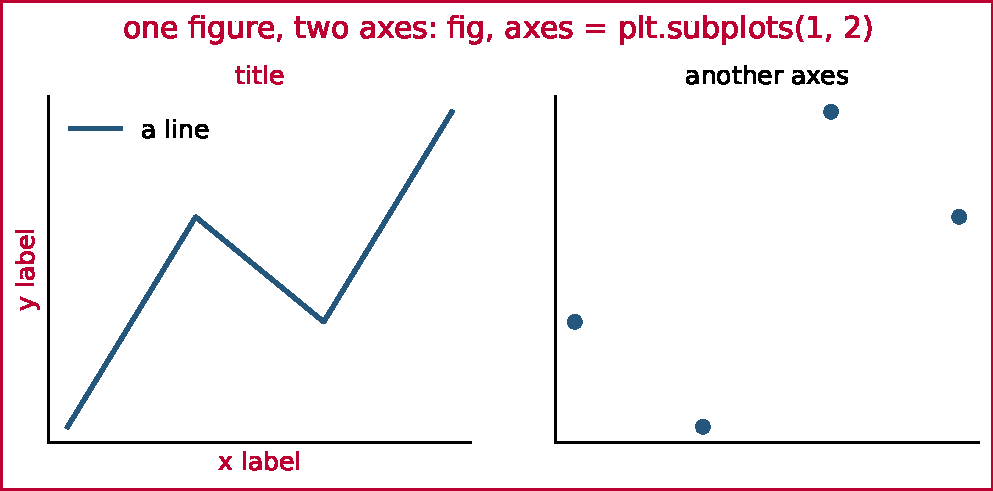
\includegraphics[width=0.62\textwidth]{l02_anatomy.pdf}

  \raggedright
  \begin{lstlisting}
fig, axes = plt.subplots(1, 2)     # 1 row, 2 columns
axes[0].plot([0, 1, 2, 3], [1, 3, 2, 4])
axes[1].scatter([1, 2, 3, 4], [2, 1, 4, 3])
  \end{lstlisting}

  \note{A figure is one window or one image file; an axes is one drawing
    area with its own coordinate system.  Every plot command is a method of
    an axes: ax.plot, ax.set\_title, and so on.  Older code calls
    plt.plot directly, which draws on the ``current'' axes; we always use
    fig, ax = plt.subplots() to keep it explicit.}
\end{frame}

\begin{frame}[fragile]{Line plot: change over time}
  \begin{columns}[T,onlytextwidth]
    \begin{column}{0.48\textwidth}
      \begin{lstlisting}
fig, ax = plt.subplots()
ax.plot(weeks, econ, marker="o",
        label="Economics")
ax.plot(weeks, psych, marker="s",
        label="Psychology")
ax.set_xlabel("week of the course")
ax.set_ylabel("study hours per week")
ax.legend()
      \end{lstlisting}
    \end{column}
    \begin{column}{0.48\textwidth}
      \centering
      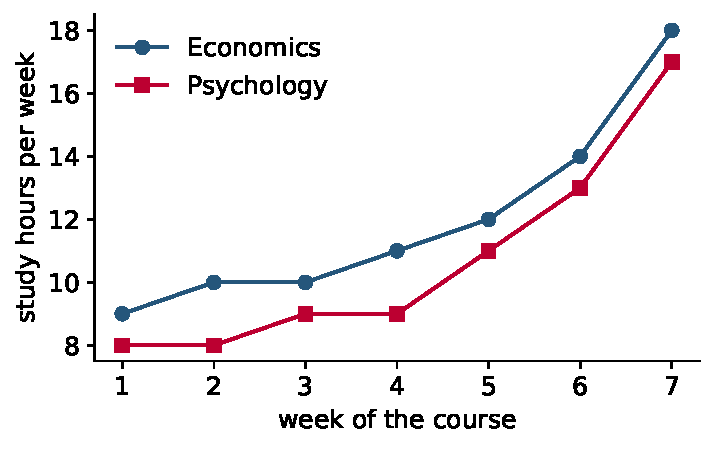
\includegraphics[width=\linewidth]{l02_line.pdf}
    \end{column}
  \end{columns}

  \note{weeks, econ and psych are three short lists of numbers, defined in
    the course script.  A line connects points in order, so use it only
    when the order of the x-axis means something, such as time.}
\end{frame}

\begin{frame}[fragile]{Scatter plot: two numbers}
  \begin{columns}[T,onlytextwidth]
    \begin{column}{0.48\textwidth}
      \begin{lstlisting}
fig, ax = plt.subplots()
ax.scatter(df["study_hours"], df["grade"],
           alpha=0.6)
ax.set_xlabel("study hours per week")
ax.set_ylabel("grade")
      \end{lstlisting}
    \end{column}
    \begin{column}{0.48\textwidth}
      \centering
      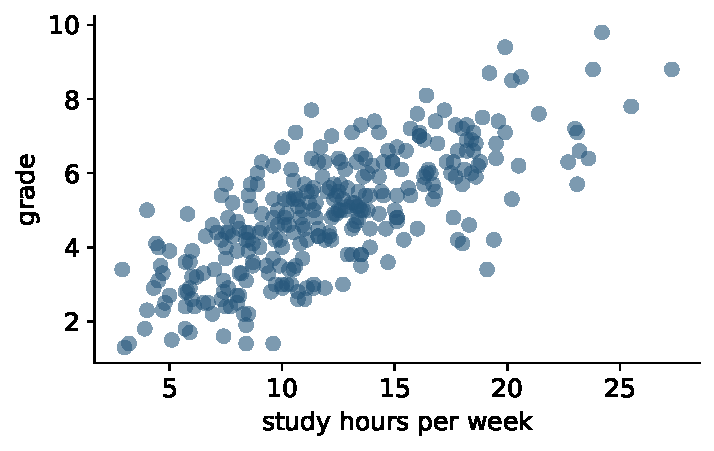
\includegraphics[width=\linewidth]{l02_scatter.pdf}
    \end{column}
  \end{columns}

  \note{Each dot is one student.  alpha makes the dots transparent, so that
    overlapping dots show as darker areas.  This is the most important plot
    for supervised learning: a feature against the label.}
\end{frame}

\begin{frame}[fragile]{Histogram: the distribution of one number}
  \begin{lstlisting}
fig, ax = plt.subplots()
ax.hist(df["sleep_hours"], bins=20)     # try bins=5 and bins=100
  \end{lstlisting}

  \centering
  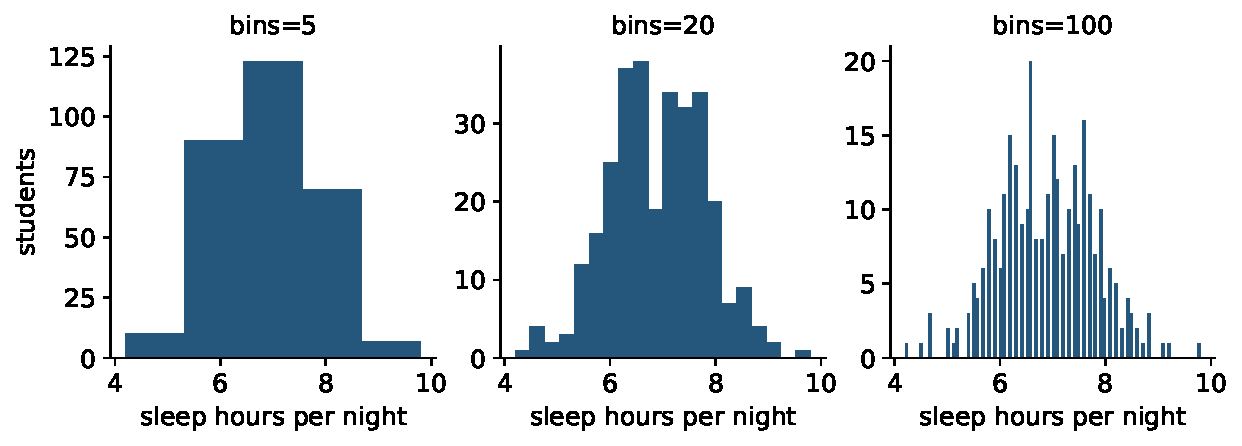
\includegraphics[width=0.85\textwidth]{l02_hist.pdf}

  \raggedright
  \muted{Too few bins hide the shape; too many show only noise.}

  \note{bins="auto" lets numpy choose a reasonable number.}
\end{frame}

\begin{frame}[fragile]{Bar chart: one number per group}
  \begin{columns}[T,onlytextwidth]
    \begin{column}{0.48\textwidth}
      \begin{lstlisting}
means = (df.groupby("program")["grade"]
           .mean().sort_values())

fig, ax = plt.subplots()
ax.barh(means.index, means.values)
ax.set_xlabel("average grade")
      \end{lstlisting}
    \end{column}
    \begin{column}{0.48\textwidth}
      \centering
      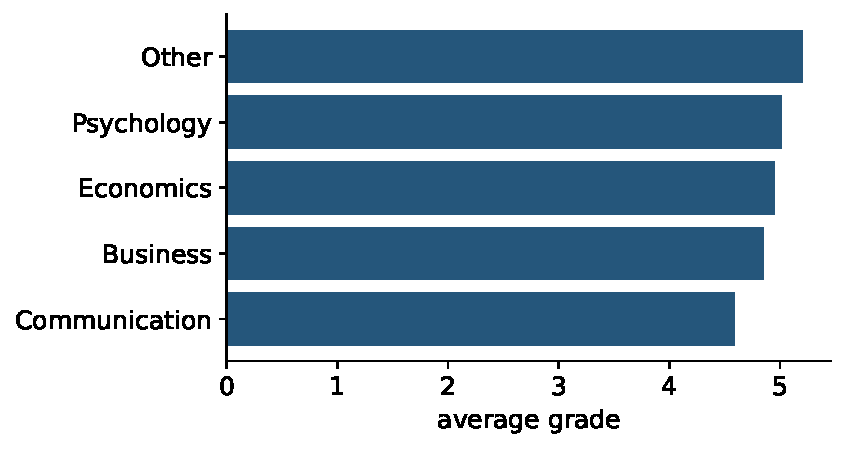
\includegraphics[width=\linewidth]{l02_bar.pdf}
    \end{column}
  \end{columns}

  \vfill
  \muted{Horizontal bars leave room for long labels; sorting makes the
  ranking visible.}

  \note{groupby splits the table by program, and mean averages the grade
    within each group.  We will meet groupby again in the labs.}
\end{frame}

\begin{frame}[fragile]{Heatmap: a table of numbers}
  \begin{columns}[T,onlytextwidth]
    \begin{column}{0.50\textwidth}
      \begin{lstlisting}
cols = ["study_hours", "social_media_hours",
        "sleep_hours", "grade"]
corr = df[cols].corr()

fig, ax = plt.subplots()
im = ax.imshow(corr, cmap="RdBu",
               vmin=-1, vmax=1)
fig.colorbar(im)
      \end{lstlisting}
    \end{column}
    \begin{column}{0.46\textwidth}
      \centering
      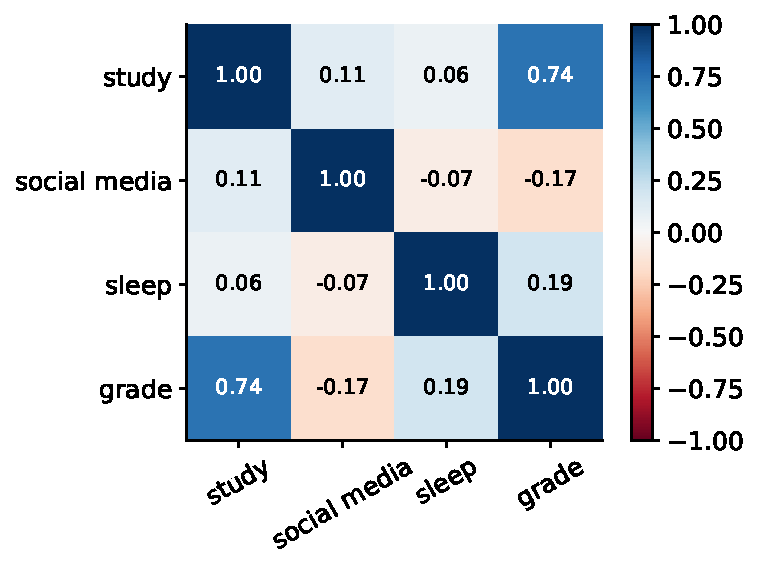
\includegraphics[width=0.9\linewidth]{l02_heatmap.pdf}
    \end{column}
  \end{columns}

  \note{A correlation lies between -1 and 1 with a natural midpoint at 0,
    so a diverging colormap fits.  vmin and vmax fix the scale, so that 0
    is always white.  Study hours correlate most strongly with the grade.}
\end{frame}

\begin{frame}[fragile]{From default to readable}
  \centering
  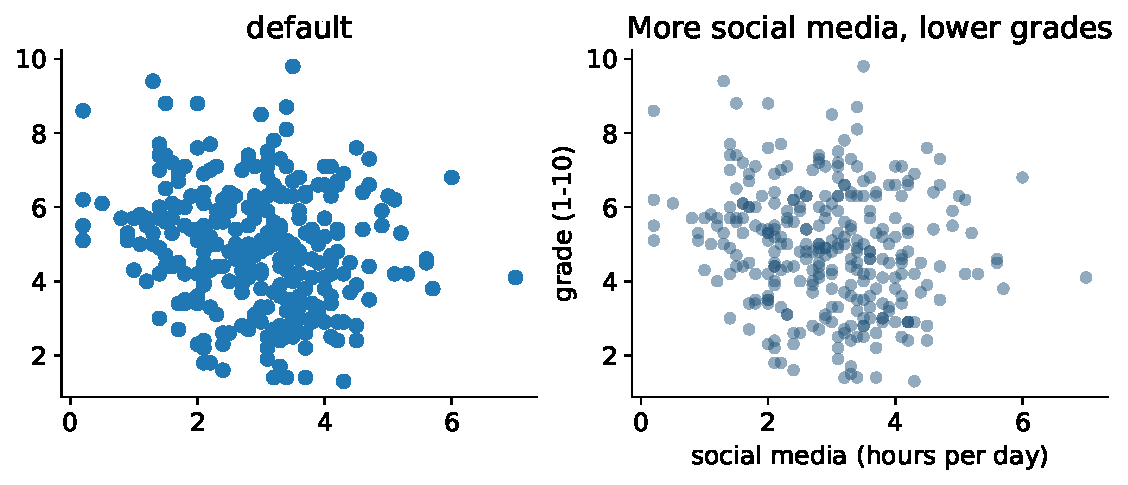
\includegraphics[width=0.8\textwidth]{l02_readable.pdf}

  \raggedright
  \begin{lstlisting}
ax.set_xlabel("social media (hours per day)")
ax.set_ylabel("grade (1-10)")
ax.set_title("More social media, lower grades")
  \end{lstlisting}

  \note{Labels with units, and a title that states the finding.  A reader
    should understand the plot without the surrounding text.}
\end{frame}

\begin{frame}[fragile]{Twin axes: use with care}
  \begin{columns}[T,onlytextwidth]
    \begin{column}{0.48\textwidth}
      \begin{lstlisting}
fig, ax1 = plt.subplots()
ax1.plot(years, phds)
ax2 = ax1.twinx()     # second y-axis
ax2.plot(years, arcades, color="red")
      \end{lstlisting}

      \vspace{0.3cm}
      \begin{itemize}
        \item Each axis has its own scale.
        \item By choosing the scales, any two rising series can be made to
              overlap.
      \end{itemize}
    \end{column}
    \begin{column}{0.48\textwidth}
      \centering
      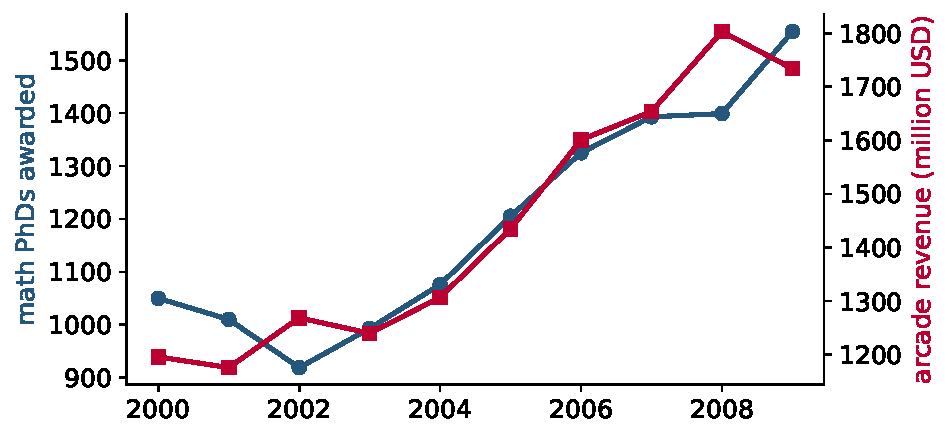
\includegraphics[width=\linewidth]{l02_spurious.pdf}
    \end{column}
  \end{columns}

  \note{This is how the correlation plot of the first session was made.
    Twin axes are useful for two quantities with different units, but
    readers compare the heights of the lines, and those heights are chosen
    by the plotter.}
\end{frame}

\begin{frame}[fragile]{seaborn: the same in one line}
  \begin{lstlisting}
import seaborn as sns
sns.scatterplot(data=df, x="study_hours", y="grade", hue="passed")
  \end{lstlisting}

  \centering
  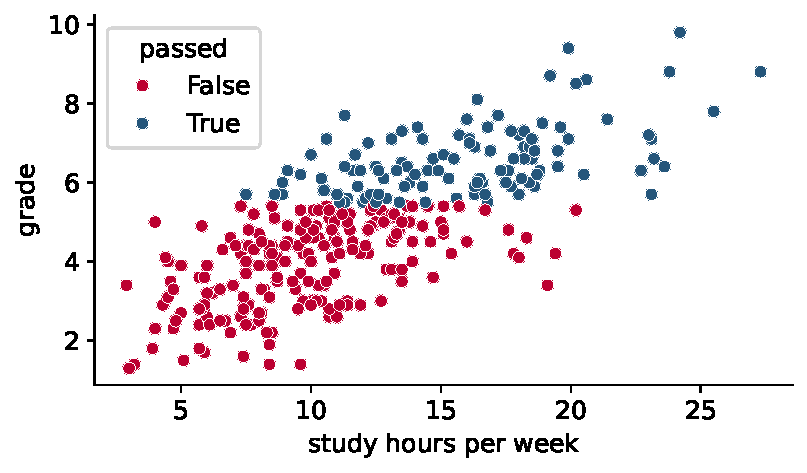
\includegraphics[width=0.6\textwidth]{l02_seaborn.pdf}

  \note{seaborn works directly with a pandas table: name the columns, and
    hue colors the points by a third column, with a legend.  The labs use
    seaborn often; underneath, it draws with matplotlib, so ax.set\_xlabel
    and the like still work.}
\end{frame}

% ==================================================================
\section{Checking Data Quality}
% ==================================================================

\begin{frame}[fragile]{Four lines before any plot}
  \begin{columns}[T,onlytextwidth]
    \begin{column}{0.52\textwidth}
      \begin{lstlisting}
raw = pd.read_csv("student_survey_raw.csv")
raw.dtypes              # types per column
raw.isna().sum()        # missing values
raw.duplicated().sum()  # duplicate rows
raw.describe()          # min, max, mean, ...
      \end{lstlisting}
    \end{column}
    \begin{column}{0.44\textwidth}
      \begin{sibbox}{In the raw survey}
        \begin{itemize}
          \item \texttt{grade} is text
          \item 28 missing values
          \item 5 duplicate rows
          \item maximum sleep: 70 hours
        \end{itemize}
      \end{sibbox}
    \end{column}
  \end{columns}

  \vspace{0.2cm}
  \centering
  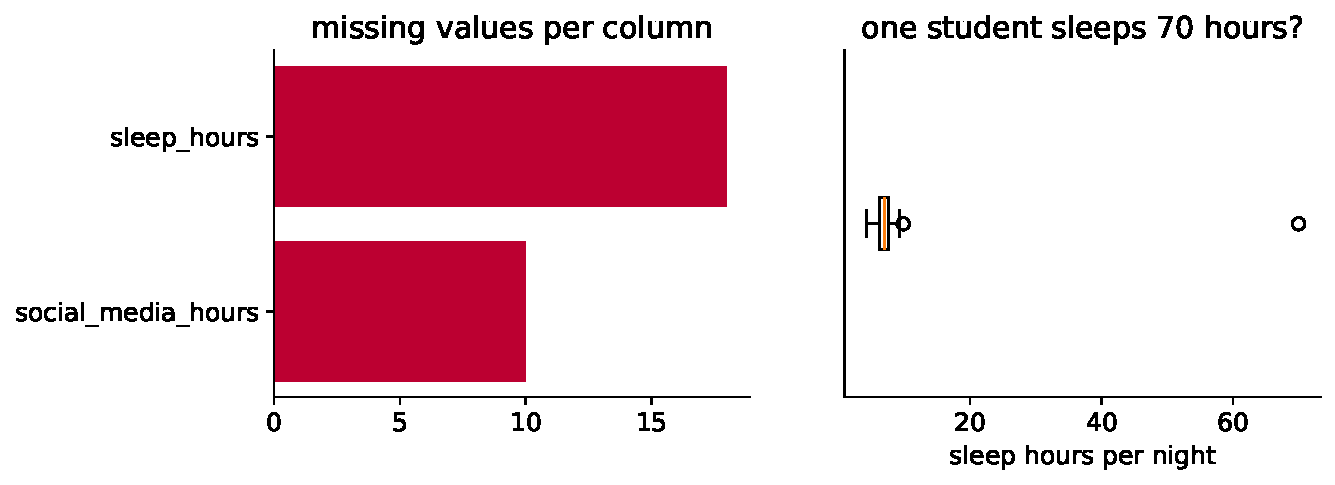
\includegraphics[height=2.9cm]{l02_quality.pdf}

  \note{The raw file is the same survey with the problems that real survey
    exports have: grades with a decimal comma, missing answers, duplicated
    submissions, typing errors (70 instead of 7.0), and some study hours per
    day instead of per week.  How to repair them is the topic of Lectures 6
    and 7.}
\end{frame}

\begin{frame}{A data-quality checklist}
  \vspace{0.2cm}
  \begin{tabular}{@{}lll@{}}
    \toprule
    \textbf{Question} & \textbf{Look at} & \textbf{Lecture} \\
    \midrule
    Right data types?           & \texttt{dtypes}               & 6 \\
    Missing values?             & \texttt{isna().sum()}, bar chart & 7 \\
    Duplicate records?          & \texttt{duplicated().sum()}   & 6 \\
    Very different scales?      & \texttt{describe()}           & 6 \\
    Outliers and typing errors? & box plot, histogram           & 13 \\
    Same definition everywhere? & histogram                     & --- \\
    Do you know what each column means? & the codebook          & --- \\
    \bottomrule
  \end{tabular}

  \vfill
  \begin{takeaway}
    Garbage in, garbage out: no model repairs data that are wrong.
  \end{takeaway}

  \note{Missing values also raise a question about bias: who did not
    answer, and why?  Column names such as ``FE1EF'' are useless without a
    codebook.}
\end{frame}

\begin{frame}{Check your understanding}
  \begin{exercise}[three exam-style questions]
    \begin{enumerate}[itemsep=3pt,topsep=3pt]
      \item Four datasets have the same means, variances and correlation.
            Then\\
            A.~their plots look alike \quad
            B.~their plots can look very different \quad
            C.~they are the same data
      \item Which colormap suits profits that can be negative or positive?\\
            A.~\texttt{jet} \quad B.~a sequential one \quad
            C.~a diverging one \quad D.~a qualitative one
      \item Which visual channel do readers judge most accurately?\\
            A.~color \quad B.~area \quad C.~angle \quad
            D.~position along a common scale
    \end{enumerate}
  \end{exercise}

  \begin{solution}
    1.~B (Anscombe's quartet).  2.~C: zero is the natural midpoint.
    3.~D.
  \end{solution}
\end{frame}

\begin{frame}{Where this is going}
  \vspace{0.3cm}
  \begin{takeaway}
    Plot the data before modeling it.  Plots reveal problems that summary
    numbers hide, and a few lines of \texttt{matplotlib} are enough.
  \end{takeaway}

  \vfill
  \begin{comingup}
    Lecture~3 (Monday, November 2): supervised learning, our first model
    ($k$-nearest neighbors), and how to test a model on new data.
  \end{comingup}

  \vfill
  \textbf{Reading.} M\"{u}ller and Guido (2016), Chapter~1: ``Essential
  Libraries and Tools'' and ``First Things First: Look at Your Data''.
\end{frame}

\begin{frame}{References}
  \scriptsize
  \begin{itemize}
    \item Anscombe, F.~J. (1973).  Graphs in statistical analysis.
          \emph{The American Statistician}, 27(1), 17--21.
    \item Borland, D. and Taylor II, R.~M. (2007).  Rainbow color map
          (still) considered harmful.  \emph{IEEE Computer Graphics and
          Applications}, 27(2), 14--17.
    \item Cleveland, W.~S. and McGill, R. (1984).  Graphical perception:
          Theory, experimentation, and application to the development of
          graphical methods.  \emph{Journal of the American Statistical
          Association}, 79(387), 531--554.
    \item Hill, K. (2016).  How an internet mapping glitch turned a random
          Kansas farm into a digital hell.  \emph{Fusion}, April 10, 2016.
          \url{https://www.jezebel.com/how-an-internet-mapping-glitch-turned-a-random-kansas-f-1793856052}
    \item Hunter, J.~D. (2007).  Matplotlib: A 2D graphics environment.
          \emph{Computing in Science \& Engineering}, 9(3), 90--95.
    \item M\"{u}ller, A.~C. (2017).  Applied Machine Learning, Lecture 3:
          Visualization and matplotlib (slides and notebook).  Columbia
          University.  \url{https://github.com/amueller/applied_ml_spring_2017}
    \item M\"{u}ller, A.~C. and Guido, S. (2016).  \emph{Introduction to
          Machine Learning with Python}.  O'Reilly Media.
    \item Rudinac, S. (2025).  Machine Learning, Lecture 2: Visualization
          and Matplotlib.  Lecture slides, University of Amsterdam.
    \item Smith, N. and van der Walt, S. (2015).  A better default colormap
          for matplotlib.  Talk at SciPy 2015.
          \url{https://www.youtube.com/watch?v=xAoljeRJ3lU}
    \item Tufte, E.~R. (1983).  \emph{The Visual Display of Quantitative
          Information}.  Graphics Press.
    \item Vigen, T.  Spurious correlations.
          \url{https://tylervigen.com/spurious-correlations}
    \item Waskom, M.~L. (2021).  seaborn: Statistical data visualization.
          \emph{Journal of Open Source Software}, 6(60), 3021.
  \end{itemize}
\end{frame}

\end{document}
